% !TeX program = xelatex
% !BIB program = bibtex
\documentclass{bistu-doctoral}
% 本地和 Overleaf 均从 fonts/ 加载 Word 要求的原字体，不使用替代字体。
\graphicspath{{figures/}}
% 在此统一填写题目、作者、学号、导师、学院、专业、方向及日期。
% 封面、题名页、声明与 PDF 题目和作者元数据读取这些配置。
\setthesisinfo
  {博士学位论文中文题目}
  {Title of the Doctoral Dissertation}
  {张三}{Zhang San}{0000000000}
  {李四 教授}{Prof. Li Si}
  {学科专业名称}{Name of the Discipline}
% 封面题目可按语义手动分行；完整题目仍使用上面的第一项。
\newcommand{\thesistitlezhcover}{博士学位论文\\中文题目}
\renewcommand{\thesisschool}{培养学院名称}
\renewcommand{\thesisdirection}{学科方向名称}
\renewcommand{\thesistype}{学术型/专业型} % 使用时选择一种。
\renewcommand{\thesischair}{王五 教授}
\renewcommand{\thesiscommittee}{王五 教授\\赵六 教授\\孙七 教授\\周八 教授}
\renewcommand{\completiondate}{20XX 年 X 月 X 日}
\renewcommand{\defensedate}{20XX 年 X 月 X 日}
\renewcommand{\submitdate}{20XX 年 X 月 X 日}
% true 显示封面“内部资料，注意保存”；false 关闭该标识。
\confidentialtrue
% 兼容旧版备注开关；通用模板的格式说明集中在第一章。
\newif\ifbistuformatnotes
\bistuformatnotesfalse

% 全部格式说明和排版示例集中在 chapters/ch01.tex，不在各页插入备注。
\hypersetup{pdftitle={\thesistitlezh},pdfauthor={\thesisauthorzh}}
\begin{document}
% 五页封面/题名/声明不显示页码，禁用页码锚点以防重名。
\hypersetup{pageanchor=false}
\pagestyle{empty}
% 三页封面/题名页。各页独立分组。
% 中文题目采用 26 bp 黑体、1.5 倍行距（32 bp 基准 × 1.5）；仅在题目段内生效。
\thispagestyle{empty}
\begingroup
\setlength{\parindent}{0pt}
% Word 首段继承两字符缩进：三号 16 磅 × 2 = 32 bp。
% 对照原始封皮 PDF：文字左端约 117 bp、上端约 75 bp。
% 只校正本行的可见位置，保持行盒尺寸，避免推动下方校徽和标题。
{\fsonggb\fontsize{16bp}{22bp}\selectfont
  \hspace*{32bp}%
  \raisebox{-3.7bp}[\height][\depth]{%
    单位代码：\raisebox{-1bp}[\height][\depth]{{\tnr 11232}}}%
  \ifconfidential
    % 原 Word 不宜公开封皮：宋体三号，右上角方框；不占正文排版空间。
    \begin{tikzpicture}[remember picture,overlay]
      \draw[line width=0.75bp]
        ([xshift=363.95bp,yshift=-74.15bp]current page.north west)
        rectangle ++(160.75bp,-26.70bp);
      \node[anchor=center,inner sep=0pt,
        font=\normalfont\songti\fontsize{16bp}{20bp}\linespread{1.5}\selectfont]
        at ([xshift=444.325bp,yshift=-87.5bp]current page.north west)
        {内部资料，注意保存};
    \end{tikzpicture}%
  \fi\par}
\vspace{1.1cm}
\begin{center}

\includegraphics[width=7cm]{bistu_logo_full.png}\par
\vspace{1.0cm}
% 【格式备注】“博士学位论文”：黑体56磅、单倍行距，独立段落居中。
{\heiti\fontsize{56bp}{64bp}\linespread{1}\selectfont 博士学位论文\par}
\vspace{0.2cm}
% 【格式备注】学位类型：黑体20磅、1.5倍行距；段落在组内结束，避免样式外溢。
{\heiti\fontsize{20bp}{24bp}\linespread{1.5}\selectfont （\thesistype）\par}
\vspace{1.8cm}
{\heiti\bfseries\fontsize{26bp}{32bp}\linespread{1.5}\selectfont\thesistitlezhcover\par}
\vspace{2.0cm}
{\fsonggb\fontsize{16bp}{30bp}\selectfont
\begin{tabular}{@{}l@{}}
培养学院：\thesisschool\\
学科专业：\thesismajorzh\\
作者姓名：\thesisauthorzh\\
指导教师：\thesissupervisorzh\\
完成日期：\completiondate
\end{tabular}\par}
\end{center}
\par\endgroup\clearpage

\thispagestyle{empty}
\begingroup
\setlength{\parindent}{0pt}
\vspace*{2.0cm}
% 【格式备注】黑体二号22磅、1.5倍行距；相邻字间一个黑体普通空格=11磅。
% 显式间隔避免xeCJK忽略中文之间的源代码空格。
{\centering\heiti\fontsize{22bp}{28bp}\linespread{1.5}\selectfont
博\hspace{11bp}士\hspace{11bp}学\hspace{11bp}位\hspace{11bp}论\hspace{11bp}文\par}
% 下面1.1cm是封面分区留白；题目自身段前、段后另各设2.5磅。
\vspace{1.1cm}
\vspace{2.5bp}
{\centering\heiti\bfseries\fontsize{26bp}{32bp}\linespread{1.5}\selectfont\thesistitlezhcover\par}
\vspace{2.5bp}
\vspace{2.5cm}
% 一个普通仿宋16磅空格=8磅；仅在本页将姓名字段中的空格显式化。
% 元数据仅展开一层，保留委员名单中的换行，不修改thesis-info.tex。
% 使用普通TeX命令，避免编辑器把LaTeX3命令名中的下划线误判为数学下标。
% 末尾空格只作分隔终止符；先选定分支再输出，允许委员名单中的换行。
\protected\long\def\bistutitleperson#1{%
  \expandafter\bistutitlespaces#1 \bistutitlespacestop}
\long\def\bistutitlespaces#1 #2\bistutitlespacestop{%
  \ifstrempty{#2}{#1}{#1\hspace{8bp}\bistutitlespaces#2\bistutitlespacestop}}
% 按Word示例将各字段左端对齐，整个信息块按最长一行的宽度居中。
% 冒号后显式空8磅，内容紧随各自字段，不强制对齐不同长度字段的冒号。
{\centering\fsong\fontsize{16bp}{30bp}\selectfont
% 保留全宽冒号，避免标点压缩改变冒号后的显式间隔。
\xeCJKsetup{PunctStyle=plain}
\begin{tabular}[t]{@{}l@{}}
作\hspace{2em}者：\hspace{8bp}\bistutitleperson{\thesisauthorzh}\\
学\hspace{2em}号：\hspace{8bp}\thesisstudentid\\
指导教师：\hspace{8bp}\bistutitleperson{\thesissupervisorzh}\\
答辩委员会主席：\hspace{8bp}\bistutitleperson{\thesischair}\\
答辩委员会委员：\hspace{8bp}\begin{tabular}[t]{@{}l@{}}\bistutitleperson{\thesiscommittee}\end{tabular}\\
学科专业：\hspace{8bp}\thesismajorzh\\
学科方向：\hspace{8bp}\thesisdirection\\
论文答辩日期：\hspace{8bp}\defensedate\\
论文提交日期：\hspace{8bp}\submitdate
\end{tabular}\par}
\par\endgroup\clearpage

\thispagestyle{empty}
\begingroup
\setlength{\parindent}{0pt}
\centering
\vspace*{1.8cm}
{\tnr\fontsize{16bp}{24bp}\selectfont
A Dissertation Submitted for the Degree of Doctor of Philosophy\par}
\vspace{3.5cm}
% 【格式备注】英文题目Times New Roman 26磅加粗、固定32磅行距；只改格式。
% 显式将行距倍率设为1，避免32磅再叠加其他段落的倍数行距。
{\normalfont\tnr\bfseries\fontsize{26bp}{32bp}\linespread{1}\selectfont\thesistitleen\par}

\vfill
{\tnr\fontsize{16bp}{30bp}\selectfont
\begin{tabular}{@{}l@{\hspace{1em}}l@{}}
Major: & \underline{\makebox[8.6cm]{\thesismajoren}}\\
Candidate: & \underline{\makebox[8.6cm]{\thesisauthoren}}\\
Supervisor: & \underline{\makebox[8.6cm]{\thesissupervisoren}}
\end{tabular}\par}
\vspace*{2.5cm}
\par\endgroup\clearpage

%========================================================
% 第4页：学位论文版权使用授权书
% 不进入目录、不显示页码
% 标题：黑体小二加粗
% 正文：宋体四号
%========================================================

\clearpage
\thispagestyle{empty}

\begingroup

%--------------------------------------------------------
% 本页正文统一设置
% 宋体四号：14bp
%--------------------------------------------------------
\songti
\fontsize{14bp}{24bp}\selectfont
\setlength{\parindent}{2em}
\setlength{\parskip}{0bp}

%--------------------------------------------------------
% 标题：黑体小二、加粗
%--------------------------------------------------------
\begin{center}
{\heiti\bfseries\fontsize{18bp}{27bp}\selectfont
学位论文版权使用授权书
\par}
\end{center}

\vspace{0.65cm}

%--------------------------------------------------------
% 正文
%--------------------------------------------------------
本人完全了解北京信息科技大学关于收集、保存、使用学位论文的规定，
按照学校要求提交学位论文的印刷本和电子版本。学校有权保留学位论文
并向国家主管部门或其指定机构送交论文的电子版和纸质版，允许论文被
查阅和借阅，可以采用影印、缩印或扫描等复制手段保存、汇编学位论文。
学校有权适当复制、公布论文的全部或部分内容。学校有权将本人的学位
论文加入《中国优秀博士学位论文全文数据库》和编入《中国知识资源总库》。

%--------------------------------------------------------
% 作者签名
%--------------------------------------------------------
\vspace{0.65cm}

\noindent
\hfill
学位论文作者签名：\hspace{2.3cm}

\par
\vspace{0.05cm}

\noindent
\hfill
年\hspace{1.5em}月\hspace{1.5em}日
\hspace{1.1cm}

%--------------------------------------------------------
% 中间虚线
%--------------------------------------------------------
\vspace{0.30cm}

\noindent
\makebox[\textwidth][c]{%
  \leaders\hbox to 0.75em{%
    \hss\raisebox{0.45ex}{\rule{0.35em}{0.35bp}}\hss
  }\hfill
}

\vspace{0.25cm}

%--------------------------------------------------------
% 公开 / 保密
%--------------------------------------------------------
\noindent
\hspace*{2em}%
$\square$公开
\hspace{2em}%
$\square$保密（\underline{\hspace{1.2cm}}年%
\underline{\hspace{1.2cm}}月）
（保密的学位论文在解密后应遵守此协议）

%--------------------------------------------------------
% 最下方签名
%--------------------------------------------------------
\vspace{0.45cm}

\noindent
\begin{minipage}[t]{0.47\textwidth}
指导教师签名：

\vspace{0.55cm}

\hfill
年\hspace{1.5em}月\hspace{1.5em}日
\end{minipage}
\hfill
\begin{minipage}[t]{0.47\textwidth}
学位论文作者签名：

\vspace{0.55cm}

\hfill
年\hspace{1.5em}月\hspace{1.5em}日
\end{minipage}

\endgroup

\clearpage
%========================================================
% 第5页：论文原创性声明

\clearpage
\thispagestyle{empty}

\begingroup


%--------------------------------------------------------
\begin{center}
\vspace*{0.35cm}

{\heiti\bfseries\fontsize{18bp}{27bp}\selectfont
博士学位论文原创性声明
\par}

\end{center}

% 标题与正文之间距离
\vspace{0.65cm}

%--------------------------------------------------------
% 正文
% 宋体四号：14bp
%--------------------------------------------------------
{\songti\fontsize{14bp}{24bp}\selectfont

\setlength{\parindent}{2em}
\setlength{\parskip}{0bp}

本人郑重声明：所呈交的论文题目为《\thesistitlezh》学位论文，
是本人在导师指导下，进行研究工作所取得的成果。尽我所知，
除了文中特别加以标注的内容外，本学位论文的研究成果不包含任何他人
创作的、已公开发表或者没有公开发表的作品的内容。对本论文所涉及的
研究工作做出贡献的其他个人和集体，均已在文中以明确方式标明
并表示了谢意。本学位论文原创性声明的法律责任由本人承担。

%--------------------------------------------------------
% 作者签字区域
% 按 Word 模板放到页面中下部
%--------------------------------------------------------
\vspace{4.20cm}

\noindent
\hspace*{8.1cm}作者签字：

\par
\vspace{0.25cm}

\noindent
\hspace*{11.2cm}年\hspace{1.6em}月\hspace{1.6em}日

}

\endgroup

\clearpage

\clearpage
\frontmatter
\hypersetup{pageanchor=true}
\bistufrontheader{摘\quad 要}
\bistuchineseabstract
此处填写中文摘要。

\cnkeywords{关键词一；关键词二；关键词三}

\clearpage
\bistufrontheader{Abstract}
\bistuenglishabstract
Replace this paragraph with the English abstract.

\enkeywords{keyword one, keyword two, keyword three}

\bistutableofcontents
\bistulistoffigures
\bistulistoftables
\bistufrontheader{符号清单}
\bistuunnumbered{符号清单}{符号清单}
\label{chap:notation}

\begingroup
\setlength{\LTleft}{\fill}
\setlength{\LTright}{\fill}
\setlength{\LTpre}{6bp}
\setlength{\LTpost}{0bp}
\renewcommand{\arraystretch}{1}
\begin{longtable}{@{}>{\centering\arraybackslash}p{2.2cm}@{\hspace{0.5cm}}>{\raggedright\arraybackslash}p{11.8cm}@{}}
\textbf{符号} & \textbf{说明} \\[6bp]
\endfirsthead
\textbf{符号} & \textbf{说明} \\[6bp]
\endhead
$x$ & 标量变量 \\
$\bistuvec{x}$ & 向量 \\
$\bistumat{A}$ & 矩阵 \\
$i$ & 元素索引 \\
$n$ & 样本数量 \\
$t$ & 时间，单位为 $\mathrm{s}$ \\
$f$ & 函数
\end{longtable}
\endgroup

\mainmatter
\bistumainheader
\chapter{绪论}
\label{chap:introduction}
% 通用模板第一章：集中式格式指南，不依赖旧格式备注开关。

\textbf{贡献者：
BISTU-Doctoral-General-Template开发过程中，主要的维护者：
高雪峰(gxf951002@163.com)：2026年10月创建BISTU-Doctoral-General-Template。
同时，也要感谢北京信息科技大学光电学院李伟仙院长与孙继超老师的大力支持！}

本章集中说明模板的使用方法、页面设置、各部分格式及图表、公式和参考文献的写法。各项说明分别依据学校模板的明确要求、模板示例的实际属性、已确认的排版要求及本模板的统一设置；示例属性与明确规范不一致时，以明确规范为准。本章的图形、符号和数值均为排版示意，不代表真实研究对象、设备参数或实验结果。正式写作时，可用实际绪论替换本章。

\section{使用方法与字体配置}

个人信息统一在 \texttt{thesis-info.tex} 中填写，包括中英文题目、姓名、学号、导师、学院、专业、方向、学位类型、答辩委员会及日期。封面、题名页、原创性声明和 PDF 元数据读取这些字段。封面题目另有分行字段，修改完整题目时应同步修改，避免内容不一致。章节顺序由 \texttt{main.tex} 管理，正文、图片和文献分别存放在 \texttt{chapters/}、\texttt{figures/} 和 \texttt{bib/} 中。

本模板使用 XeLaTeX 与 BibTeX。手动编译顺序为 XeLaTeX、BibTeX、XeLaTeX、XeLaTeX；BibTeX 的目标为 \texttt{main}。也可运行工程中的构建脚本，或使用 \verb|latexmk -xelatex main.tex|。在 Overleaf 中将主文件设为 \texttt{main.tex}，编译器设为 XeLaTeX，并保留完整字体目录。模板不使用 Biber；已由文献宏包配置引用功能，不要重复加载 \texttt{biblatex}、\texttt{natbib} 或 \texttt{cite}。

中文正文使用宋体 SimSun，标题使用黑体 SimHei；普通仿宋与封面所需的仿宋\_GB2312分别加载。英文及数字主要使用 Times New Roman，英文摘要标题使用 Arial。所有字体均从 \texttt{fonts/} 中读取，缺失时应补齐原字体，不使用替代字体。字号与间距使用 \texttt{bp}，即每磅为 $1/72$ 英寸，对应 Word 的磅值；不要将其与 TeX 的 \texttt{pt} 混用。

\section{页面、页眉、页码与起排规则}

纸张为 A4，上下边距均为 2.54 厘米；每页固定左边距 3 厘米、右边距 2.5 厘米，装订线为 0。模板采用双面排版，奇偶页不交换左右边距。页眉及页脚距纸边均为 2 厘米。

页眉居中、不加粗，中文为宋体五号（10.5 磅），英文和数字为 Times New Roman 10.5 磅，1.5 倍行距，下设 0.4 磅横线。前置部分显示所在部分名称；正文与后置部分右页显示“北京信息科技大学博士学位论文”，左页显示当前章序号与章名，无编号部分只显示名称。英文摘要的页眉为 Times New Roman 10.5 磅。

页码位于页脚中央，通常为宋体五号（10.5 磅），英文摘要部分改用 Times New Roman 10.5 磅。封面和中英文题名页共三页，另有两页声明，这五页不显示页眉、页码。中文摘要从大写罗马数字 I 开始，英文摘要、目录、图表清单和符号清单连续排页，不逐项为右开插入空白页。正文从阿拉伯数字 1 开始连续编号。

正文各章、无编号结论及后置部分从右页开始。为此补出的空白左页仍保留当前部分的页眉、横线及居中页码，并参与连续计数；它通常承接上一章的页眉。打印时应保留这些空白页，维持左右页关系。固定左右边距、双面页眉与右页起排是同时生效的设置。

\section{封面、题名页与声明}

\subsection{中文封面与题名页}

封面“博士学位论文”为黑体 56 磅、单倍行距，学位类型为黑体 20 磅、1.5 倍行距，分别成段居中。中文论文题目为黑体 26 磅，加粗居中、1.5 倍行距。单位代码及培养学院、学科专业、作者姓名、指导教师、完成日期五行中文使用仿宋\_GB2312三号（16 磅），英文和数字使用 Times New Roman。学校单位代码为 11232。

中文题名页的“博士学位论文”为黑体二号（22 磅）、1.5 倍行距，相邻字间留一个普通空格，模板显式设置为 11 磅。题目为黑体 26 磅、加粗居中、1.5 倍行距，段前、段后各 2.5 磅。信息中文使用普通仿宋三号（16 磅），信息块按最长一行的宽度整体居中，各字段左端对齐；内容紧随各自字段，冒号后及姓名与“教授”之间各留一个普通空格（8 磅）。委员续行与首位委员姓名的左端对齐。本页不显示页眉、页码。

\subsection{英文题名页与封面标记}

英文题目采用 Times New Roman 26 磅，加粗居中、固定 32 磅行距；英文说明和个人信息为 16 磅，个人信息行距为 30 磅。本页不显示页眉、页码。

封面右上角可显示“内部资料，注意保存”。标记为宋体三号（16 磅）、1.5 倍行距，矩形框尺寸为 $160.75\times26.70$ 磅，框线宽 0.75 磅，位置沿用模板。\verb|\confidentialtrue| 显示标记，\verb|\confidentialfalse| 隐藏标记。此开关只控制封面提示文字和外框，不替代授权书中的公开或保密选项。

\subsection{版权使用授权书与原创性声明}

两页声明保留学校规定的正文措辞和待签区域，不列入目录，也不显示页眉、页码。现有模板中，标题为黑体小二（18 磅）加粗、27 磅基线间距；正文为宋体四号（14 磅）、24 磅行距、首行缩进两个汉字符、段前后 0 磅。这些数值为模板页面的实际样式属性。原创性声明的论文题目读取统一配置；公开或保密选项、签名和日期应按实际情况填写。

\section{摘要、目录与各类清单}

\subsection{中文摘要及关键词}

“摘”与“要”之间空一格，标题为黑体二号（22 磅）加粗居中、单倍行距，下空一行排正文。正文采用宋体小四（12 磅），两端对齐、首行缩进两个汉字符（24 磅）、20 磅行距，段前后 0 磅。摘要之后空一正文行排关键词，字号为小四，“关键词”加粗；各词用分号分隔，最后一个词后不加标点。

摘要应说明基本研究内容、研究方法、创造性成果及理论和实际意义。一般不使用公式、图表或文献引用编号，不写成目录式介绍，不加入领域常识、应在引言中展开的内容或自我评价。表达应简明、准确、结构严谨，一般采用第三人称；可直接使用“对……进行了研究”等句式，不必以“本文”或“作者”作主语。

\subsection{英文摘要及关键词}

英文摘要标题 Abstract 使用 Arial 16 磅、加粗居中、单倍行距，段前 24 磅、段后 18 磅。正文为 Times New Roman 12 磅、20 磅行距，两端对齐、首行缩进 24 磅、段前后 0 磅，内容与中文摘要一致。关键词前空两正文行（40 磅），采用 Times New Roman 12 磅；“KEY WORDS”加粗，关键词小写、用逗号分隔，末词后不加标点。

\subsection{目录、插图清单与表格清单}

目录标题为黑体三号（16 磅）加粗居中、单倍行距，段前 24 磅、段后 18 磅。各级条目为宋体小四（12 磅）、单倍行距，段前 6 磅、段后 0 磅，两端对齐、页码右对齐。章条目不缩进，一级节左缩进一个汉字符（12 磅），二级节缩进两个汉字符（24 磅）。模板默认列到二级节，如 1.2.1；三级节如 1.2.1.1 可以编号，但默认不列入目录。

插图清单和表格清单标题沿用模板示例属性：黑体二号（22 磅）加粗居中、单倍行距，段前 24 磅、段后 18 磅；条目为宋体小四、单倍行距，段前 6 磅、段后 0 磅，页码右对齐。目录和图表清单均自动生成，不手工填写编号或页码。

\subsection{符号清单}

符号清单位于图表清单之后、正文之前，并列入目录。标题沿用章标题格式，清单文字沿用正文小四号格式。左侧为符号，右侧为含义及必要单位；不加边框、横线、表号或项目编号。符号字形应与正文及公式一致；增加或改变公式中的符号时，应同步更新定义和单位。

\section{标题、段落与脚注}

章标题为黑体二号（22 磅），加粗居中、单倍行距，段前 24 磅、段后 18 磅，章序号与章名之间空一个本字号的汉字符（22 磅）。一级节标题为黑体三号（16 磅），二级节为黑体四号（14 磅），三级节为黑体小四（12 磅）；均加粗左齐、单倍行距，段前 24 磅、段后 6 磅，编号与题名间分别空 16、14、12 磅。二级节对应三段编号，三级节对应四段编号。节标题中的数字沿用 Times New Roman 粗体，章标题数字使用黑体。

正文中文为宋体小四，英文为 Times New Roman 12 磅，两端对齐，首行缩进两个汉字符（24 磅），20 磅行距，段前后 0 磅；标题后的首段也保留缩进。连续标题之间按段前与段后的较大值处理，例如节标题连续出现时保留 24 磅，不将 6 磅与 24 磅相加。各级节标题自然换页至页首时，仍保留 24 磅段前间距，不用手工空行或负间距调整位置。段前间距属于正文排版区内的段落设置，不等于标题文字与页眉横线之间的距离。

随文脚注为宋体小五（9 磅），使用带圈数字，全文跨章连续编号。\footnote{此处为脚注格式示例，仅用于展示带圈编号、宋体小五字号及正文脚注的位置。} 不应手工输入脚注序号。普通段落不要用双反斜杠命令强行换行；标题和题注的编号间距由模板控制，不额外插入空格模拟。

表\ref{tab:word-format-requirements}集中保留学校 Word 模板“论文写作规范”的九类项目。表内“示例”只演示编号形式；字号和间距适用于对应的论文元素，说明表本身不按章、节标题字号放大。
% 学校 Word 模板“论文写作规范”的九类项目，集中由第一章载入。
% 普通正文，不依赖旧格式备注开关；采用 longtable 以允许自然分页。
\par
\begingroup
\bistutablefont
\setlength{\tabcolsep}{5bp}
\setlength{\heavyrulewidth}{1.5bp}
\setlength{\lightrulewidth}{0.75bp}
\setlength{\LTleft}{\fill}
\setlength{\LTright}{\fill}
\renewcommand{\arraystretch}{1.2}
\begin{longtable}{@{}C{2.2cm}C{2.8cm}C{9.6cm}@{}}
  \caption{论文写作规范}\label{tab:word-format-requirements}\\
  \toprule
  \textbf{项目} & \textbf{示例} & \textbf{要求} \\
  \midrule
  \endfirsthead
  % 使用真正的续表题注，继承表题段前/段后各6磅；空可选参数不重复进入清单。
  \caption[]{论文写作规范（续）}\\
  \toprule
  \textbf{项目} & \textbf{示例} & \textbf{要求} \\
  \midrule
  \endhead
  \bottomrule
  \endfoot
  各章标题 & 第1章\quad ××× & 黑体二号加粗居中，单倍行距，段前24磅，段后18磅，章序号与章名间空一个汉字符 \\[6bp]
  一级节标题 & 1.3\quad ××× & 黑体三号加粗，左齐，单倍行距，段前24磅，段后6磅，序号与题名间空一个汉字符 \\[6bp]
  二级节标题 & 1.3.1\quad ××× & 黑体四号加粗，左齐，单倍行距，段前24磅，段后6磅，序号与题名间空一个汉字符 \\[6bp]
  三级节标题 & 1.3.1.1\quad ×× & 黑体小四加粗，左齐，单倍行距，段前24磅，段后6磅，序号与题名间空一个汉字符 \\[6bp]
  段落文字 & \shortstack{××××××\\××××××} & 宋体小四（英文用Times New Roman体12磅），两端对齐书写，段落首行左缩进2个汉字符。行距20磅；段落中有数学表达式时，可根据表达需要设置该段行距。段前0磅，段后0磅 \\[6bp]
  随文脚注 & \circlednum{1}××× & 宋体小五，全文连续编号 \\[6bp]
  图序、图名 & 图2.1\quad ××× & 置于图的下方，宋体五号居中，单倍行距，段前6磅，段后12磅，图序与图名文字之间空一个汉字符 \\[6bp]
  表序、表名 & 表3.1\quad ××× & 置于表的上方，宋体五号居中，单倍行距，段前6磅，段后6磅，表序与表名文字之间空一个汉字符 \\[6bp]
  表达式 & （3.2） & 序号加圆括号，右顶格排，单占行 \\
\end{longtable}
\endgroup


\section{图、表与自动引用}

\subsection{图片、图题与子图示例}

图序和图名置于图下方，采用宋体五号（10.5 磅）、居中、单倍行距，段前 6 磅、段后 12 磅，图序与图名之间空一个汉字符（10.5 磅）。图、表、公式分别独立按章编号，新章从 1 开始，格式为“章.序号”。图题的段前后间距与浮动体到相邻正文的距离是不同参数，不应混为一项。

图\ref{fig:generic-panels}使用原生绘图展示通用的 $2\times2$ 子图排列。子图标记放在各自图形下方，整图题注位于所有子图之后；本例不依赖额外的子图宏包。正式论文应按实际内容替换图形、子图名称及尺寸。

\begin{figure}[htbp]
  \centering
  \begin{minipage}[t]{0.46\textwidth}
    \centering
    \begin{tikzpicture}[x=0.8cm,y=0.8cm]
      \path[use as bounding box] (-0.2,-0.2) rectangle (4.6,3.0);
      \draw[rounded corners=2pt] (0.2,0.45) rectangle (1.4,1.55);
      \draw[rounded corners=2pt] (2.6,0.45) rectangle (3.8,1.55);
      \node at (0.8,1) {$x$};
      \node at (3.2,1) {$y$};
      \draw[->,thick] (1.5,1) -- (2.5,1);
    \end{tikzpicture}\par
    {\bistutablefont (a) 输入与输出\par}
  \end{minipage}\hfill
  \begin{minipage}[t]{0.46\textwidth}
    \centering
    \begin{tikzpicture}[x=0.8cm,y=0.8cm]
      \path[use as bounding box] (-0.2,-0.2) rectangle (4.6,3.0);
      \draw[->] (0.4,0.2) -- (3.9,0.2) node[right] {$x$};
      \draw[->] (0.4,0.2) -- (0.4,2.0) node[above] {$y$};
      \draw[thick] (0.7,0.5) -- (1.5,0.8) -- (2.4,1.2) -- (3.5,1.7);
      \foreach \x/\y in {0.7/0.5,1.5/0.8,2.4/1.2,3.5/1.7}
        \fill (\x,\y) circle (1.5pt);
    \end{tikzpicture}\par
    {\bistutablefont (b) 变化趋势示意\par}
  \end{minipage}
  \par\vspace{8bp}
  \begin{minipage}[t]{0.46\textwidth}
    \centering
    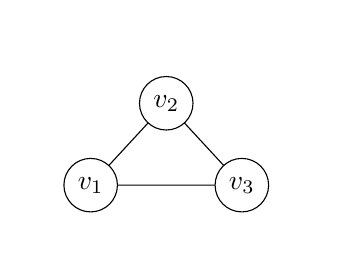
\begin{tikzpicture}[x=0.8cm,y=0.8cm]
      \path[use as bounding box] (-0.2,-0.2) rectangle (4.6,3.0);
      \draw (0.8,0.5) -- (2,1.8) -- (3.2,0.5) -- cycle;
      \foreach \x/\y/\n in {0.8/0.5/1,2/1.8/2,3.2/0.5/3}
        \node[circle,draw,fill=white,inner sep=3pt] at (\x,\y) {$v_{\n}$};
    \end{tikzpicture}\par
    {\bistutablefont (c) 连接关系示意\par}
  \end{minipage}\hfill
  \begin{minipage}[t]{0.46\textwidth}
    \centering
    \begin{tikzpicture}[x=0.8cm,y=0.8cm]
      \path[use as bounding box] (-0.2,-0.2) rectangle (4.6,3.0);
      \draw (0.7,0.4) rectangle (3.3,1.9);
      \draw (2,0.4) -- (2,1.9);
      \draw (0.7,1.15) -- (3.3,1.15);
      \node at (1.35,1.525) {$a_{11}$};
      \node at (2.65,1.525) {$a_{12}$};
      \node at (1.35,0.775) {$a_{21}$};
      \node at (2.65,0.775) {$a_{22}$};
    \end{tikzpicture}\par
    {\bistutablefont (d) 矩阵结构示意\par}
  \end{minipage}
  \caption{通用图形与子图排列示例（示意图）}
  \label{fig:generic-panels}
\end{figure}

图的 \verb|\caption| 放在图形之后，\verb|\label| 紧随题注，正文通过 \verb|\ref| 自动引用。更改图序后，正文引用和插图清单随重新编译更新；子图的字母标记与整图的章内编号分别维护。

\subsection{表题与三线表示例}

表序和表名置于表上方，宋体五号（10.5 磅）、居中、单倍行距，段前后各 6 磅，序号与表名之间空一个汉字符（10.5 磅）。按已确认要求采用三线表，无竖线，单元格内容水平及垂直居中；表内中文宋体、英文和数字 Times New Roman，均为五号。顶线、底线为 1.5 磅，表头分隔线为 0.75 磅；线宽是本模板统一设置，并非原 Word 的明确规定。

表\ref{tab:generic-data}演示普通及双行单元格。可用 \texttt{bistuthreelinetabular} 环境和 \verb|C{宽度}| 列型，分别以 \verb|\toprule|、\verb|\midrule|、\verb|\bottomrule| 生成三条横线。表的题注在表格前，标签紧随题注；不要整体缩放表格，否则会同时改变文字字号。

\begin{table}[htbp]
  \centering
  \caption{通用测量数据排版示例（虚构数据）}
  \label{tab:generic-data}
  \begin{bistuthreelinetabular}{@{}C{2.2cm}C{3.3cm}C{3.4cm}C{3.2cm}@{}}
    \toprule
    样本 & 条件说明 & 长度 $l$ / $\mathrm{m}$ & 时间 $t$ / $\mathrm{s}$ \\
    \midrule
    A & \shortstack{条件一\\重复测量} & 1.20 & 2.40 \\
    B & 条件二 & 1.50 & 3.00 \\
    C & 条件三 & 1.80 & 3.60 \\
    \bottomrule
  \end{bistuthreelinetabular}
  \par\smallskip
  {\bistutablefont 注：全部数值为虚构的排版示例，不作为实验结果。\par}
\end{table}

\section{公式、数学字形与局部行距}

公式单独成行，序号加圆括号并右顶格排，使用 \texttt{equation} 环境编号；正文以 \verb|\eqref| 引用。拉丁和希腊变量采用 Times New Roman 斜体，向量和矩阵采用粗斜体；数字、函数名、单位及说明性上下标为正体，变量索引为斜体。求和、积分、伸缩括号、根号和花体字母等使用专用数学字形，不能统称为 Times New Roman。

% 高矩阵示例与引导句一起排版，预留完整公式及其下方间距。
\Needspace{6\baselineskip}
普通标量可直接输入 $x_i$、$a_{ij}$、$\alpha$；向量用 \verb|\bistuvec|，矩阵用 \verb|\bistumat|，两者也支持希腊字母。下式演示标量、向量和矩阵的关系：
\begin{equation}
  \bistuvec{y}=\bistumat{A}\bistuvec{x},\qquad
  \bistuvec{x}=\begin{pmatrix}x_1\\x_2\end{pmatrix},\qquad
  \bistumat{A}=\begin{pmatrix}a_{11}&a_{12}\\a_{21}&a_{22}\end{pmatrix}.
  \label{eq:generic-vector-matrix}
\end{equation}
% 预留解释句及上下标示例的高度，避免高公式挤到页脚附近。
\Needspace{5\baselineskip}
\noindent 式\eqref{eq:generic-vector-matrix}中的下标 $i,j$ 和各标量元素保持斜体；数字保持正体。迭代索引 $k$ 采用斜体，表示最大值、转置等含义的上下标用 \verb|\mathrm|：
\begin{equation}
  0\leq x_i^{(k)}\leq x_i^{\mathrm{max}},\qquad
  q=\bistuvec{x}^{\mathrm{T}}\bistuvec{x},\qquad
  v=1.2\,\mathrm{m}\,\mathrm{s}^{-1}.
  \label{eq:generic-scripts-units}
\end{equation}
单位前留适当间隔，函数使用 \verb|\sin|、\verb|\exp| 等正体命令，不将函数名当成多个相乘变量。函数和最小化目标的示例为
\begin{equation}
  f(\alpha)=\sin\alpha+\exp(-\alpha),\qquad
  \min_{\bistuvec{x}}\sum_{i=1}^{n}(x_i-y_i)^2.
  \label{eq:generic-functions}
\end{equation}

普通正文保持 20 磅行距，含较高行内表达式的段落可局部放宽行距。使用环境 \texttt{bistumathparagraph}，以可选参数 \verb|[24bp]| 指定 24 磅行距；只调整确有需要的段落。下段给出效果示例。

\begin{bistumathparagraph}[24bp]
本段使用 24 磅行距，以容纳较高的行内分式 $\dfrac{x_1+x_2}{1+\alpha^2}$。字号仍为小四，首行缩进和段距沿用正文设置；表达式仅用于说明局部行距的用法。
\end{bistumathparagraph}

环境结束后，普通段落自动恢复 12 磅字号、20 磅行距。数学符号在正文、图表和符号清单中应保持相同字形及含义。

\section{参考文献与著录示例}

参考文献标题同章标题：黑体二号（22 磅）加粗居中、单倍行距，段前 24 磅、段后 18 磅。条目中文宋体小四，英文 Times New Roman 12 磅，两端对齐、20 磅行距、段前后 0 磅，条目间不额外空行；模板设置的悬挂量为 24 磅。

文献采用顺序编码制，按正文首次引用顺序编号，重复引用沿用原编号。\verb|\cite{文献键}| 输出上标方括号引用，\verb|\inlinecite{文献键}| 输出行内引用。文献数据库为 \texttt{bib/} 目录内的 \texttt{references.bib}，由随工程提供的 \texttt{bistu-thesis.bst} 与 BibTeX 生成列表。不要手工填写序号，也不要编辑自动生成的 \texttt{.bbl} 文件。通常只列出被引用条目；确有需要时使用单条 \verb|\nocite{文献键}|。本通用模板的参考文献页使用该命令展示十类虚构演示文献；正式写作时应删除演示条目及其展示命令，按实际引用生成文献列表。

作者之间用 \texttt{and} 分隔，中文姓名可额外用花括号保持完整；语言字段控制“等”或“et al.”，超过三位作者保留前三位后加省略标记。译者填 \texttt{translator}，学校填 \texttt{school}，报告机构填 \texttt{institution}，出版地或授予地填 \texttt{address}，出版者填 \texttt{publisher}。页码如 \verb|10--18| 输出为起～止页码；类型标记自动生成，不写进题名。

期刊、专著、会议论文、学位论文分别可用 \texttt{article}、\texttt{book}、\texttt{inproceedings}、\texttt{phdthesis} 等 BIB 类型。网上文章用 \texttt{online}，网址填 \texttt{url}，日期填 \texttt{date}。本样式按学校示例定制，不自动追加 DOI 或访问日期，普通文献也不会仅因填写网址就自动改变类型标记。完整字段说明见工程中的 BIB 格式说明文档；所有正式条目均应核对实际来源。

% 学校模板的10类标识和8种著录示意，集中由第一章载入。
% 字段占位不是实际文献，不进入 BibTeX 列表；不受旧备注开关控制。
\subsection{十种文献类型标识}

学校模板列示的类型为：期刊文章[J]，专著[M]，论文集[C]，学位论文[D]，报告[R]，标准[S]，专利[P]，网上文章[EB/OL]，报纸文章[N]，论文集中的析出文献[A]。整本论文集与其中的析出文献应按实际来源选择类型。

\subsection{八种著录格式示意}

以下保留学校模板列示的八种著录格式。“序号”“作者”“题名”等均是字段占位，不是真实文献信息，不加入实际参考文献列表，也不参与其编号。报告和析出文献属于上述类型清单；它们未被另行计作学校原表的八种示例。

\noindent\textbf{期刊文章：} [序号] 作者. 文章名[J]. 刊名（外文期刊可缩写），年，卷号（期号）：起～止页码。

\noindent\textbf{专（译）著：} [序号] 作者. 书名[M]. （译者，译）. 出版地：出版者，出版年. 起～止页码。

\noindent\textbf{论文集：} [序号] 作者. 题名. 论文集名[C]. 出版地：出版者，出版年. 起～止页码。

\noindent\textbf{学位论文：} [序号] 姓名. 论文题目[D]. 授予地：授予单位，授予年。

\noindent\textbf{专利：} [序号] 申请者. 专利名：国名，专利号[P]. 出版日期。

\noindent\textbf{网上文章：} [序号] 作者，文章名[EB/OL]. 文章出处或可获得网址，发表或更新日期。

\noindent\textbf{技术标准：} [序号] 发布单位. 技术标准编号. 技术标准名称[S]. 出版地：出版者，出版日期。

\noindent\textbf{报刊文章：} [序号] 作者. 文章名[N]. 报刊名，出版日期（版次）。


\section{结论、致谢与个人简历}

结论单独从右页起排，列入目录，但不显示“第几章”。结论、致谢和个人简历与学术成果的标题均沿用章标题格式，即黑体二号（22 磅）加粗居中、单倍行距，段前 24 磅、段后 18 磅。正文采用宋体及 Times New Roman 12 磅、20 磅行距、两端对齐、首行缩进 24 磅、段前后 0 磅。无编号结论的内部标题使用无编号形式，不沿用前一章的节编号。

结论应是论文最终和总体的结论，做到明确、精练、完整、准确，着重阐述作者的创造性工作及成果在本领域的地位、作用与意义，严格区分本人、他人和导师的研究成果。还应评价应用前景及社会、经济价值，提出需要讨论的问题和建议。可从论文总结、主要创新点、研究局限与展望等方面组织，结论必须有已完成工作的证据支持。

致谢按实际帮助填写。个人简历与学术成果须以真实情况为依据；成果独立编号，不与参考文献混编，不得将演示条目列为真实成果。

\section{集中说明与开关}

本章全部说明和示例为普通正文，不受旧格式备注开关影响。原来分散在各页的格式备注已集中迁入本章，旧备注入口已移除。\verb|\bistuformatnotesfalse| 仅为兼容旧工程而保留；即使将它改为真，也不会重新恢复逐页备注。需要修改或删除集中说明时，应直接编辑本章内容。

封面标记仍由 \verb|\confidentialtrue| 或 \verb|\confidentialfalse| 独立控制，与集中说明及旧备注开关无关。使用已有的真、假命令切换，不重复定义开关，也不要只在命令前加注释符号而省略明确状态。

修改内容、开关或章节结构后，应重新编译，使目录、图表清单、交叉引用和页码更新；通常至少再运行两次 XeLaTeX，涉及文献时还需运行 BibTeX。调整封面标记不会改变页面边距、正文右页起排以及补白页的页眉、页码规则。正式提交前，应替换通用占位信息、示例图表和虚构数据，并逐项核对实际论文。

\chapter{预备知识}
\label{chap:preliminaries}
\section{基本概念}
此处填写研究所需的基本概念。
\section{理论基础}
此处填写相关理论基础。
\section{本章小结}
此处填写本章小结。

\chapter{研究方法一}
\label{chap:method-one}
\section{引言}
此处填写本章引言。
\section{问题描述}
此处填写研究问题。
\section{方法设计}
此处填写研究方法。
\section{实验结果与分析}
此处填写实验结果与分析。
\section{本章小结}
此处填写本章小结。

\chapter{研究方法二}
\label{chap:method-two}
\section{引言}
此处填写本章引言。
\section{问题描述}
此处填写研究问题。
\section{方法设计}
此处填写研究方法。
\section{实验结果与分析}
此处填写实验结果与分析。
\section{本章小结}
此处填写本章小结。

\chapter{研究方法三}
\label{chap:method-three}
\section{引言}
此处填写本章引言。
\section{问题描述}
此处填写研究问题。
\section{方法设计}
此处填写研究方法。
\section{实验结果与分析}
此处填写实验结果与分析。
\section{本章小结}
此处填写本章小结。

\chapter{系统设计与验证}
\label{chap:system}
\section{系统需求}
此处填写系统需求。
\section{总体设计}
此处填写系统总体设计。
\section{系统实现}
此处填写系统实现内容。
\section{测试与验证}
此处填写测试结果与分析。
\section{本章小结}
此处填写本章小结。

\bistuunnumbered{结论}{结论}
\section*{研究工作总结}
此处填写研究工作总结。
\section*{主要贡献}
此处填写主要贡献。
\section*{研究局限与展望}
此处填写研究局限与展望。

\backmatter
\bistubackheader{参考文献}
% 以下十条仅用于展示书目类型；正式写作时替换为实际引用文献。
\begingroup
\renewcommand{\bibpreamble}{以下条目为虚构的格式示例，不可作为真实文献引用。\par}
\nocite{demoJournal,demoTranslation,demoConference,demoThesis,demoReport,demoStandard,demoPatent,demoOnline,demoNews,demoContribution}
\bibliographystyle{bistu-thesis}
\bibliography{bib/references}
\endgroup

% 先补白再切换页眉，保证空白左页仍属于上一部分。
\cleardoublepage
\bistubackheader{致\quad 谢}
\chapter*{致\quad 谢}
\addcontentsline{toc}{chapter}{致谢}
感谢导师李四教授的指导，感谢王五、赵六等同学的帮助与支持。

\cleardoublepage
\bistubackheader{个人简历、博士学位期间发表的学术成果}
\chapter*{个人简历、博士学位期间发表的学术成果}
\addcontentsline{toc}{chapter}{个人简历、博士学位期间发表的学术成果}

\begingroup
\songti
\fontsize{12bp}{20bp}\selectfont
\setlength{\parindent}{2em}
\setlength{\parskip}{0pt}
\justifying

张三，20XX 年 X 月出生，籍贯名称。于 20XX 年 X 月在学校名称获得学位名称，专业为专业名称。主要研究方向为研究方向名称。

博士学位期间发表的学术成果有：

\begin{enumerate}[
  label={[\arabic*]},
  leftmargin=4em,
  labelwidth=2em,
  labelsep=0.5em,
  align=left,
  itemindent=0pt,
  listparindent=0pt,
  itemsep=0pt,
  parsep=0pt,
  topsep=0pt,
  partopsep=0pt
]
\item 张三，李四．论文题目示例[J]．期刊名称，20XX，卷号(期号)：起页--止页．
\item 张三，李四．论文题目示例．会议论文集名称[C]．出版地：出版者，20XX．起页--止页．
\item 张三，李四．专利名称示例：中国，专利号[P]．20XX-XX-XX．
\end{enumerate}
\endgroup

\end{document}
